\section{ToaruOS}

\begin{figure}[H]
    \centering
    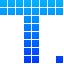
\includegraphics[width=0.4\textwidth]{figures/logoToaruOS.png}
    \caption[Ícono de ToaruOS]
            {Ícono de ToaruOS \citep{toaruoslogo2025}}
    \label{fig:ToaruOS}
\end{figure}

ToaruOS creado en 2010 por Kevin Lange, es un sistema operativo experimental con fines educativos, que busca evidenciar cómo se puede desarrollar un entorno completo desde la nada, independiente de kernels o librerías existentes. Su intención primigenia fue servir como soporte de investigación y aprendizaje para la comprensión del formato y funcionamiento interno de un sistema operativo moderno, incorporando subsistemas gráficos, de red y de usuario. A diferencia de proyectos como Linux o BSD, ToaruOS busca ser un entorno accesible para la enseñanza y la experimentación, y no un sistema de producción \citep{toaruos2025}.

La arquitectura de ToaruOS es híbrida. Esto significa que el kernel es en gran medida monolítico por lo que, incluye directamente los módulos significativos del sistema, como la administración de memoria, procesos, controladores de dispositivos y el sistema de archivos, pero incluye características de microkernel como la posibilidad de ejecución modular. Este diseño posibilita la integración y el rendimiento en un entorno practico. El lenguaje de implementación es C, con cantidades inferiores en ensamblador para interrelaciones de bajo nivel con el hardware y el arranque \citep{toaruos2025}.

Los elementos nucleares del sistema comprenden los elementos básicos de cualquier sistema operativo contemporáneo. Para la gestión de procesos pone en práctica tareas múltiples planificadas basada en prioridades, de igual manera de resistir hilos ligeros. Para la gestión de memoria abarca paginación, segmentación y asignación dinámica de memoria para los programas de usuario. Al respecto del sistema de archivos, dispone de su peculiar implementación denominada “tmpfs” para sistemas en memoria, asimismo la compatibilidad con EXT2 en versiones más actuales. Por otra parte, cuenta con un sistema gráfico completo, compuesto por un servidor de ventanas (Toaru Window Server), un gestor de ventanas y librerías gráficas que permiten ejecutar aplicaciones con interfaces gráficas, como un editor de texto o un navegador web básico \citep{toaruos2025}.

La comunidad de ToaruOS es reducida en comparación con otros proyectos de código abierto, pero se mantiene activa en torno a su repositorio en GitHub, donde se documentan los cambios y se comparten implementaciones experimentales. La documentación disponible proviene principalmente de su creador, quien mantiene guías, el repositorio en Github y un blog explicativo sobre su evolución. Se ha mencionado grosso modo en limitadas ocasiones en artículos científicos de especialidad.